\chapter{Architecture du projet}

%architecture pour affichage via directfb

L'affichage de la liseuse se fait grâce aux modules suivant : 
\begin{itemize}
	\item le driver mxc_epdc
	\item DirectFB
\end{itemize}~\\

Le driver se charge de faire les optimisation pour pallier au problème de réactivité de l'écran (via les tables LuTs notamment), ainsi que l'application des waveforms pour l'affichage sur l'écran.\\
Le driver fournit des ioctl pour permettre l'exécution des fonctionnalités du driver depuis l'espace utilisateur.~\\~\\
%verifier si c'est pas deja dis plus tot dans le rapport
DirectFB implémente des primitives graphique, comme le traçage de ligne. Ces dernières permettent de faire une abstraction sur le format du framebuffer.

Voici un schéma modulaire de l'application utilisant DirectFB : 

\begin{figure}[h!]
	\begin{center}	
		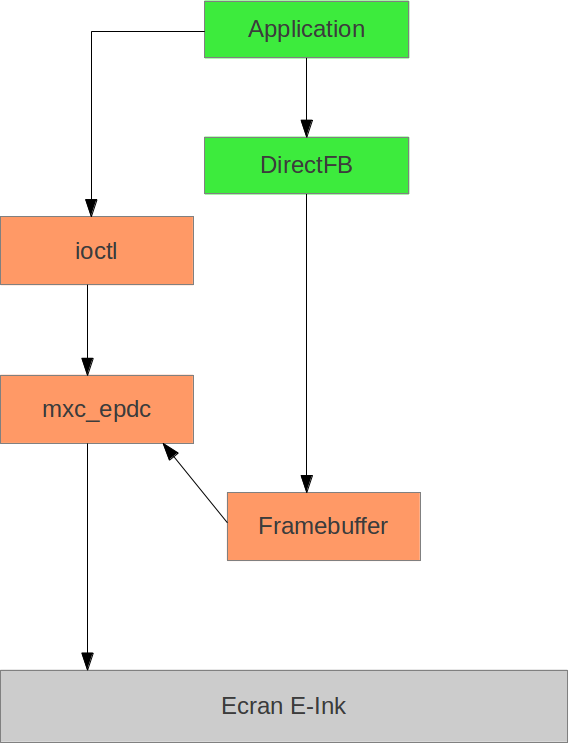
\includegraphics[scale=0.5]{schema_direct_fb.png}
		\caption{Architecture modulaire de l'application}
	\end{center}
\end{figure}

Dans l'état d'avancement actuel du projet, le programme met à jour le framebuffer via DirectFB et fait un appel ioctl au driver qui actualise l'écran en fonction du buffer. 
% application => directfb => framebuffer 				=> affichage
%						 => ioctl 	=> driver epdc   ||


%explication du fonctionnement 

% description de chaque module 
% directfb : abstraction du driver d'affichage
% ioctl : appel de la maj driver
%
%framebuffer